\section{Experiments}
    \begin{frame}{MNIST dataset}
      \begin{itemize}
      \item {MNIST, handwritten digits, has a training set of 60,000 examples, and a test set of 10,000 examples.}
      \item {The digits have been size-normalized and centered in a fixed-size image to 28x28(784) image. }
      \item {10,000 examples in 60,000 training set are used as validation set and left 50,000 images are used for training.}
      \item {The original labels values are 0 to 9 but it is vectorized by one-hot encoding.}
      \end{itemize}
      \begin{center}
    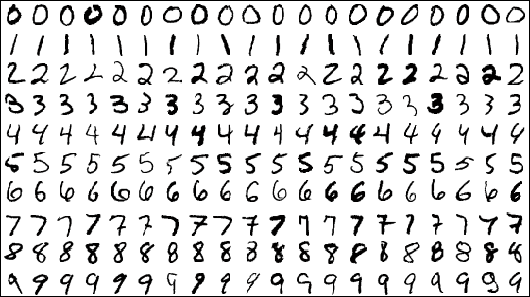
\includegraphics[width=2.4in]{mnist.png}
      \end{center}
    \end{frame}
    
\begin{frame}{Experiment parameters}
  \begin{itemize}
       \item{ \textbf{Network structures} }
				\begin{center}
				  \begin{tabular}{ | l | c | c | c | }
				    \hline
				      & \cellcolor[gray]{0.85} \# Layers & \cellcolor[gray]{0.85} \# Nodes & \cellcolor[gray]{0.85} Bias \\
				      & \cellcolor[gray]{0.85} (In,\textbf{Hidden},Out) & \cellcolor[gray]{0.85} (In,\textbf{Hidden},Out) &\cellcolor[gray]{0.85}  \\ \hline
				    Network1 & 1,\textbf{1},1 & 784,\textbf{1024},10 & Yes \\ \hline 
				    Network2 & 1,\textbf{2},1 & 784,\textbf{1024,1024},10 & Yes \\
				    \hline
				  \end{tabular}
				\end{center}
				
    \item{ \textbf{Hyperparameters} }
    \begin{center}
				  \begin{tabular}{ | c | c | c | c | }
				    \hline
				      \cellcolor[gray]{0.85} Learning Rate & \cellcolor[gray]{0.85} \# Epochs & \cellcolor[gray]{0.85} Size of Batch & \cellcolor[gray]{0.85} Regularization \\ \hline
				      0.1 & Let Me Know & $2^n$, $n\in[7,12]$ & None \\
				    \hline
				  \end{tabular}
				\end{center}
     \item{ \textbf{Activation function}}
     \begin{itemize}
      		\item{Sigmoid function}
      		\begin{align*}
      		& \sigma(z)=\frac{1}{1+e^{-z}}\\
      		& \sigma'(z)=\sigma(z)(1-\sigma(z))
      		\end{align*}
    \end{itemize}
  \end{itemize}
\end{frame}


\begin{frame}{Parallel experiments}
	\begin{itemize}
	\item { \textbf{PThreads} }
		\begin{itemize}
		\item {About PThreads setting}
		\end{itemize}
	\item { \textbf{CUDA} }
		\begin{itemize}
		\item {About CUDA setting}
		\end{itemize}
	\item { \textbf{theano} }
		\begin{itemize}
		\item {About theano}
		\end{itemize}
	\end{itemize}

\end{frame}